% SPDX-License-Identifier: Apache-2.0
%
% The TxHDL specification, as an IEEE two-column article.
% Built by //docs:article. See docs/document-build-plan.md.
\documentclass[journal,9pt]{IEEEtran}

% Two columns: listings at 6pt fit 70 columns.
\newcommand{\listingsize}{\fontsize{6}{7}\selectfont}
% SPDX-License-Identifier: Apache-2.0
%
% The house preamble, shared by every document in this directory. Loaded
% after \documentclass, before \title. Keeping it in one file is what
% stops two articles drifting apart in font, listing style or figure
% style.
% Computer Modern. IEEEtran selects Times (ptm) by default, so the face has
% to be chosen explicitly.
%
% Latin Modern is the Computer Modern variety used here, and the choice is
% forced rather than aesthetic. Under T1 encoding, plain `cmr` has no Type 1
% outlines unless cm-super is installed, and it is not in the pinned
% distribution, so pdflatex falls back to EC bitmaps and every glyph in the
% PDF becomes a Type 3 font. That was measured: the first build produced a
% document with 10 Type 3 fonts and no Type 1. Latin Modern is Computer
% Modern redrawn with a full T1 repertoire and real .pfb outlines, so the
% same design comes out scalable.
\usepackage[T1]{fontenc}
\usepackage[utf8]{inputenc}
\usepackage{lmodern}
% microtype is not in the pinned TeX distribution. emergencystretch alone
% keeps the two-column measure from producing overfull lines.
\setlength{\emergencystretch}{3em}

\usepackage{amsmath}
\usepackage{amssymb}
\usepackage{amsthm}
\usepackage{booktabs}
\usepackage{array}
% enumitem is not in the pinned TeX distribution; the list spacing below
% does what \setlist would have done.
\usepackage{float}
\usepackage{xcolor}
\usepackage{listings}
\usepackage{tikz}
\usetikzlibrary{arrows.meta,positioning,fit,backgrounds,calc}
\usepackage[hidelinks,bookmarks=true]{hyperref}

% Numbered, definition-style box for a rule the reader is meant to apply.
\theoremstyle{definition}
\newtheorem{rulebox}{Rule}
\newtheorem{example}{Example}

% Unnumbered asides.
\theoremstyle{remark}
\newtheorem*{tip}{Tip}
\newtheorem*{pitfall}{Pitfall}

% Tighter lists, in place of enumitem's \setlist.
\setlength{\topsep}{2pt}
\setlength{\itemsep}{1pt}
\setlength{\parsep}{0pt}

% Code in the running text. The typewriter face under T1 ligates `<<`
% and `>>` into guillemets, so a shift printed as \code{<<} came out as
% a French quotation mark (issue 571). microtype's \DisableLigatures is
% not in the pinned distribution, but the primitive it rests on is
% pdfTeX's own: \pdfnoligatures strips every ligature from the font it
% is given, and the current font inside \texttt is the typewriter face
% at the size in use, so each size is stripped the first time \code
% sets it. Code wants no ligature at all: two quotes are two quotes.
\newcommand{\code}[1]{\texttt{\ifdefined\pdfnoligatures\pdfnoligatures\font\fi #1}}
\newcommand{\term}[1]{\emph{#1}}

% Syntax highlighting. Four roles, distinguishable in colour and still
% distinguishable in greyscale, because an IEEE article gets printed: the
% keyword is the only bold role, the comment is the only italic one, and the
% two remaining roles differ in lightness as well as in hue.
\definecolor{kwblue}{RGB}{20,60,150}
\definecolor{cmtgreen}{RGB}{90,120,90}
\definecolor{strred}{RGB}{150,50,40}
\definecolor{numgray}{gray}{0.45}
\definecolor{framegray}{gray}{0.70}
\definecolor{bgshade}{gray}{0.97}
% A darker fill for figure cells. The listing background has to stay very
% light to keep code readable; a figure cell has to be clearly shaded or the
% distinction it draws is invisible in print.
\definecolor{cellshade}{gray}{0.90}

% The listing size is the document's choice, because it depends on the
% column: a two-column article sets `\listingsize` to 6pt and keeps its
% listings within 70 columns, or to 5.6pt when it includes source that
% rustfmt sets at 80, which is what fits a column's frame (issue 1061);
% a one-column document keeps the body size and includes source files
% at 80. `//docs:frame_test` checks every listing line against its frame. Lines are never broken; a line that does not fit
% overflows the frame, which is visible, rather than wrapping, which is
% not.
\providecommand{\listingsize}{\scriptsize}

% `'` is deliberately not a string delimiter: the language uses it for loop
% labels, as Rust does, so treating it as a quote would swallow the rest of
% the line.
\lstdefinestyle{txhdl}{
  basicstyle=\ttfamily\listingsize,
  keywordstyle=\bfseries\color{kwblue},
  commentstyle=\itshape\color{cmtgreen},
  stringstyle=\color{strred},
  numberstyle=\tiny\color{numgray},
  morekeywords={mod,use,pub,const,type,struct,enum,trait,impl,fn,async,let,mut,
    match,if,else,loop,while,for,in,break,continue,return,as,await,
    module,bus,channel,transaction,protocol,pipeline,flow,seq,config,
    port,stage,pipe,instance,connect,bind,tag,domain,blackbox,foreign,
    property,role,signal,handler,true,false,
    sequence,interface,modport,implements,package,import,var,wire,func,proc,
    case,default,next,fork,branch,join,state,fsm},
  morecomment=[l]{//},
  morestring=[b]",
  showstringspaces=false,
  columns=fullflexible,
  keepspaces=true,
  breaklines=false,
  % Framed, so a listing is bounded rather than floating in the column.
  frame=single,
  rulecolor=\color{framegray},
  framesep=3pt,
  backgroundcolor=\color{bgshade},
  xleftmargin=3pt,
  xrightmargin=3pt,
  aboveskip=6pt,
  belowskip=6pt,
  % Every listing is numbered and captioned, so it can be referred to by
  % number. `caption` without `float` numbers the listing and leaves it
  % where it was written, which is what a listing in running prose needs.
  captionpos=b,
  abovecaptionskip=2pt,
  belowcaptionskip=6pt,
}

% Figures drawn as text. Framed the same way, and with the highlighting
% switched off, because a box-and-arrow diagram is not code and half its
% words turning blue reads as an accident. Setting a style adds keys rather
% than clearing the ones already set, so the three roles are neutralised by
% hand rather than by leaving them out. Program output is printed in this
% style too, and a netlist's assignment can run past the frame, so a line
% that does not fit is broken and the rest indented; source never is.
\lstdefinestyle{ascii}{
  basicstyle=\ttfamily\listingsize,
  keywordstyle=\ttfamily,
  commentstyle=\ttfamily,
  stringstyle=\ttfamily,
  columns=fullflexible,
  keepspaces=true,
  breaklines=true,
  breakindent=2em,
  frame=single,
  rulecolor=\color{framegray},
  framesep=3pt,
  backgroundcolor=\color{bgshade},
  xleftmargin=3pt,
  xrightmargin=3pt,
  aboveskip=6pt,
  belowskip=6pt,
}
\lstset{style=txhdl}

% House TikZ styles. `shorten` lives on the arrow styles rather than on each
% arrow, so every arrow in the document gets the gap, including ones added
% later. TikZ clips a path at a node's border, so without it an arrowhead
% butts against the box with no gap at all. Keep `node distance` well above
% twice the shorten, or the arrow shrinks to nothing.
\tikzset{
  box/.style={draw,rounded corners=2pt,align=center,inner sep=4pt,
              font=\footnotesize},
  boxf/.style={box,fill=bgshade},
  lbl/.style={font=\scriptsize\itshape,align=center},
  fl/.style={-{Stealth[length=4pt]},shorten >=2.5pt,shorten <=2.5pt},
  fld/.style={fl,dashed},
}


% The contents list: the class gives a section's number 2.75em, which
% a Roman numeral past thirty overruns onto the title, so the box is
% wider here, and a subsection's entry starts where a title does.
\makeatletter
\def\l@section#1#2{\addpenalty{\@secpenalty}\addvspace{1.0em plus 1pt}%
    \@tempdima 5.75em \begingroup \parindent \z@ \rightskip \@pnumwidth%
    \parfillskip-\@pnumwidth {\bfseries\leavevmode #1}\hfil\hbox to\@pnumwidth{\hss #2}\par%
    \endgroup}
\def\l@subsection{\@dottedtocline{2}{5.75em}{5em}}
\def\l@subsubsection{\@dottedtocline{3}{10.75em}{5.5em}}
\makeatother


\InputIfFileExists{buildstamp.tex}{}{}
\providecommand{\buildstamp}{Draft build (outside the Bazel flow).}

\title{TxHDL: Unifying a Dataflow and a Transaction Hardware Description
Language}

\author{Filip Filmar and Dragiša Janković%
\thanks{Both authors are independent. Filip Filmar is the
corresponding author, at f@hdlfactory.com; Dragiša Janković is
reached at linkedin.com/in/dragisa-jankovic.}%
\thanks{This article states the merged TxHDL specification. It consolidates
two hardware description languages that were developed independently, LHDL
and TxHDL, into one. The analysis behind each decision is in the project
repository under \code{docs/}.}%
\thanks{The authors used a large language model, Claude, as an
assistant in exploring the concepts and in writing and constructing
the documents and the programs; every commit of the repository says
so and records the prompts that led to it, verbatim.}%
\thanks{\buildstamp}}

\markboth{TxHDL Specification}{Filmar and Janković: TxHDL}

\begin{document}
\maketitle

\begin{abstract}
Two hardware description languages were developed independently for the same
project. LHDL describes dataflow and leaves time to the compiler: the
designer never counts cycles, and synchronisation tags tell the compiler
where to put registers. TxHDL describes transactions over buses and lets a
module block for as many cycles as a protocol takes. We show that the two do
not compete. Each is nearly silent where the other is detailed: LHDL has no
construct for writing a multi-cycle protocol body, and TxHDL has no
interface, no late binding and no configuration facet. Four questions needed
a decision about meaning rather than spelling, and we resolve all four. The
merged language keeps both models of time and states which one a construct
belongs to. Its surface syntax follows Rust, which removes six defects that
the two source specifications had, including two grammars that their own
examples did not parse against.
\end{abstract}

\begin{IEEEkeywords}
Hardware description languages, high-level synthesis, latency-insensitive
design, language specification, dataflow, transaction-level modelling.
\end{IEEEkeywords}

{\footnotesize\tableofcontents}

% SPDX-License-Identifier: Apache-2.0
\section{Introduction}
\label{sec:introduction}

\IEEEPARstart{T}{wo} hardware description languages were developed
independently for the same project, each targeting the same underlying
hardware platform. The goal of this effort is a unified, consistent
language specification. This article defines the required consolidation
and resolves every open architectural and syntactic question.

Fundamentally, the two languages address complementary abstraction levels
rather than competing models. LHDL specifies system-level composition,
static configuration, and dataflow scheduling, leaving low-level protocol
timing to the compiler. TxHDL specifies cycle-accurate transaction protocols
and multi-cycle bus interactions within individual modules. Each language is
largely silent where the other provides fine detail. Four fundamental
questions require semantic decisions rather than superficial syntactic
alignment; Section~\ref{sec:conflicts} resolves each one.

\subsection{Source Material}

Seven repository files document language content, spanning initial sketches
to detailed drafts.

\begin{table*}[t]
\caption{The source material. Two languages, seven files, four spellings of
the name.}
\label{tab:sources}
\centering
\footnotesize
\begin{tabular}{@{}lrll@{}}
\toprule
Path & Lines & Language & What it is \\
\midrule
\code{spec/language.md}                  & 2241 & TxHDL & The complete TxHDL specification, 20 numbered sections \\
\code{filmil/workspace/draft-spec.md}    & 1218 & LHDL  & The long LHDL draft, prose plus EBNF \\
\code{filmil/workspace/spec.md}          &  486 & LHDL  & A condensed LHDL specification with a consolidated grammar \\
\code{filmil/workspace/lhdl-proposal.md} &  178 & LHDL  & The earliest LHDL sketch \\
\code{filmil/theses.md}                  &   94 & LHDL  & The twelve design theses the language argues from \\
\code{proposal.md}                       &   27 & both  & A prior agent's read of the repository and its next steps \\
\code{README.md}                         &    1 & none  & One sentence naming the two authors \\
\bottomrule
\end{tabular}
\end{table*}

Prior to this consolidation, the most comprehensive specification in the
repository was neither integrated into the automated build nor published.
The complete specification in \code{spec/language.md} lacked a build target,
whereas several smaller exploratory files possessed active Bazel rules.

Nomenclature also diverged across these documents. The extended LHDL draft
uses FLHDL 88 times; the condensed specification uses it 9 times; the initial
proposal uses LHdl 6 times; and \code{spec/language.md} introduces TxHDL 5
times. Because the repository, build targets, and distribution packages use
\code{txhdl}, Section~\ref{sec:decisions} adopts TxHDL as the canonical name.

\subsection{Contributions}

\begin{enumerate}
  \item An account of what each language actually specifies, and of the
        asymmetry that makes a merge possible rather than a compromise
        (Section~\ref{sec:two-languages}).
  \item Resolutions for the four semantic conflicts, of which the model of
        time is the one that shapes the language
        (Section~\ref{sec:conflicts}).
  \item A surface syntax biased toward Rust, decided construct by
        construct, which removes six defects present in the sources rather
        than restating them (Section~\ref{sec:syntax}).
  \item An inventory of every defect found by reading the two sources,
        with line numbers, including sixteen places where the LHDL grammar
        and the LHDL examples disagree
        (Section~\ref{sec:defects}).
\end{enumerate}

% SPDX-License-Identifier: Apache-2.0
\section{What Each Language Is}
\label{sec:two-languages}

\subsection{LHDL: dataflow, and time as an implementation detail}

LHDL starts from twelve theses. The eighth is the one that shapes the
language: at the design level there should be no notion of combinational
versus sequential logic. The designer writes dataflow and never counts
cycles, and the compiler decides where registers go.

The mechanism is the \term{tag}. A tag names a synchronisation domain.
Operations sharing a tag are aligned by the compiler through longest path
analysis, which inserts bridge registers into the shorter paths. Adding
\code{with handshake} makes the domain elastic: the compiler replaces
flip-flops with skid buffers and wires ready and valid across the whole
domain. Adding \code{capacity=32} makes the compiler generate a scoreboard
that tracks up to 32 transactions in flight and asserts backpressure when
full.

The organising idea is the \term{three facets}. The design facet states
logic and contracts and is timeless. The implementation facet maps logic
onto fabric and handles retiming. The configuration facet binds
implementations into sockets, sets generic parameters, maps tags onto
physical clocks, and links foreign code. Changing the target fabric edits
the configuration facet and leaves the design facet untouched.

Reuse runs through \term{interfaces} with \term{modports}. An interface
declares fields, and a modport names a role and gives each field a direction
for that role. A module, a pipeline or a state machine can implement an
interface.

Verification is delegated. LHDL adds no non-synthesisable subset. The
configuration facet instead binds an interface to a foreign implementation
in Go, Rust or C++, and the compiler generates a gRPC bridge and bit-exact
software structs.

\subsection{TxHDL: transactions, and time written down}

TxHDL starts elsewhere. Communication between modules happens through
transactions over buses, never through raw signals. Inside a module one
sequential flow is easy to reason about, while modules run in parallel.
Variables become registers based on how they are used.

The mechanism is \code{await}. A sequence blocks until a transaction
arrives, until a condition holds, or for a stated number of cycles.
\code{select} waits on several events and takes the first. A timeout bounds
the wait. A protocol that takes 40 cycles reads as 40 lines of straight
code rather than as a state enumeration.

Communication runs through \term{buses} made of \term{channels}, each with
implicit valid and ready handshaking. A channel marked \code{tagged by id}
matches responses to requests out of order, and a \code{then} clause
registers a callback that fires when the matching response arrives.

Typing is \term{structural}. Two transactions with the same fields are
compatible whatever their names, and a transaction with extra fields can be
sent where fewer are expected.

Verification is native. Assertions, assumptions, cover points and
properties are in the language, and properties use temporal operators.

\subsection{The asymmetry}

Four of the seven concerns in Figure~\ref{fig:asymmetry} are worked out on
both sides. The three that are not decide the merge, and each is thin on a
different side.

LHDL has no way to write a protocol body. Its state machine is a hand
written state enumeration, which is the form \code{await} exists to remove.
TxHDL has no way to assemble a system. Its top level offers instances,
connections and an address-decoding bus, and there is no interface, no late
binding, no configuration facet, no way to wrap legacy Verilog and no way to
swap an implementation.

\begin{figure*}[t]
\centering
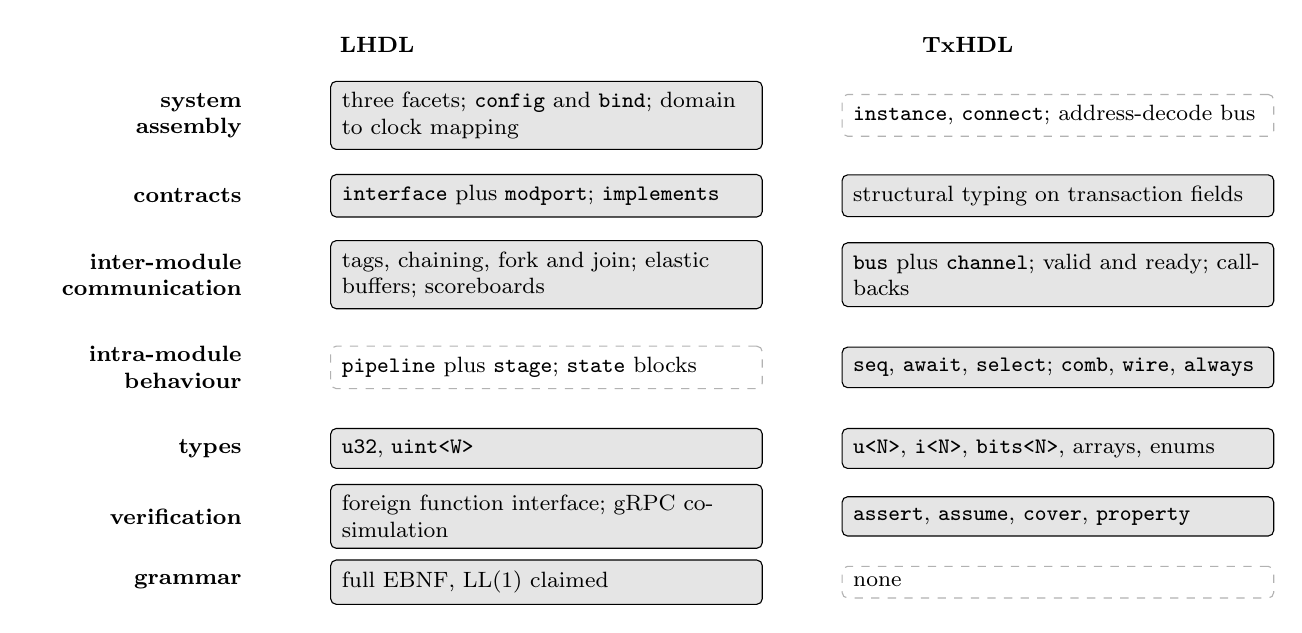
\begin{tikzpicture}[
    node distance=4mm and 10mm,
    row/.style={font=\footnotesize\bfseries,align=right,text width=26mm},
    cell/.style={box,text width=52mm,align=left},
    % Two channels, not one. An IEEE article gets printed and photocopied,
    % and a 3 per cent grey difference does not survive that. A worked-out
    % mechanism is shaded and solid; one that is only named is unshaded and
    % dashed, so the distinction reads even with the fill gone.
    thin/.style={cell,fill=white,draw=framegray,dashed},
    thick/.style={cell,fill=cellshade,draw=black},
  ]

  \node[font=\footnotesize\bfseries] (hl) at (0,0) {LHDL};
  \node[font=\footnotesize\bfseries,right=62mm of hl] (ht) {TxHDL};
  \node[row,left=10mm of hl] (h0) {};

  \node[row] (r1) at ($(h0)+(0,-9mm)$) {system\\assembly};
  \node[thick,right=10mm of r1] (l1)
    {three facets; \code{config} and \code{bind}; domain to clock mapping};
  \node[thin,right=10mm of l1] (t1)
    {\code{instance}, \code{connect}; address-decode bus};

  \node[row,below=of r1] (r2) {contracts};
  \node[thick,right=10mm of r2] (l2)
    {\code{interface} plus \code{modport}; \code{implements}};
  \node[thick,right=10mm of l2] (t2)
    {structural typing on transaction fields};

  \node[row,below=of r2] (r3) {inter-module\\communication};
  \node[thick,right=10mm of r3] (l3)
    {tags, chaining, fork and join; elastic buffers; scoreboards};
  \node[thick,right=10mm of l3] (t3)
    {\code{bus} plus \code{channel}; valid and ready; callbacks};

  \node[row,below=of r3] (r4) {intra-module\\behaviour};
  \node[thin,right=10mm of r4] (l4)
    {\code{pipeline} plus \code{stage}; \code{state} blocks};
  \node[thick,right=10mm of l4] (t4)
    {\code{seq}, \code{await}, \code{select}; \code{comb}, \code{wire},
     \code{always}};

  \node[row,below=of r4] (r5) {types};
  \node[thick,right=10mm of r5] (l5)
    {\code{u32}, \code{uint<W>}};
  \node[thick,right=10mm of l5] (t5)
    {\code{u<N>}, \code{i<N>}, \code{bits<N>}, arrays, enums};

  \node[row,below=of r5] (r6) {verification};
  \node[thick,right=10mm of r6] (l6)
    {foreign function interface; gRPC co-simulation};
  \node[thick,right=10mm of l6] (t6)
    {\code{assert}, \code{assume}, \code{cover}, \code{property}};

  \node[row,below=of r6] (r7) {grammar};
  \node[thick,right=10mm of r7] (l7) {full EBNF, LL(1) claimed};
  \node[thin,right=10mm of l7] (t7) {none};

\end{tikzpicture}
\caption{Where each language is detailed. A shaded cell is a worked-out
mechanism; an unshaded one is named and not specified. Four rows are worked
out on both sides. The three that are not, system assembly, intra-module
behaviour and the grammar, are the ones that make the merge possible: each
is thin on one side and thick on the other, and the thin side differs.}
\label{fig:asymmetry}
\end{figure*}

% SPDX-License-Identifier: Apache-2.0
\section{The Four Real Conflicts}
\label{sec:conflicts}

Everything else the two languages disagree about is spelling, and
Section~\ref{sec:syntax} settles spelling. These four need a decision about
meaning.

\subsection{Does the designer count cycles?}

LHDL says no. TxHDL says yes, and a UART example counts baud intervals
explicitly.

\begin{rulebox}[Both, with a boundary]
The two answers apply to different things, and the conflict disappears once
that is stated. A UART's baud interval is a specification: it comes from the
protocol on the wire, and a compiler that retimed it would break the design.
An adder's latency is not a specification: it comes from the fabric, and a
compiler that fixed it by hand would waste the fabric.
\end{rulebox}

The merged language therefore has two behavioural forms and a rule for
choosing between them.

\begin{itemize}
  \item \term{Timeless form}, spelled \code{flow}, from LHDL. Dataflow and
        tags, no cycle counts. The compiler schedules it, and a cycle count
        written inside one is a compile error.
  \item \term{Sequenced form}, spelled \code{seq}, from TxHDL. Explicit
        ordering with \code{await}. Cycle counts are honoured exactly as
        written.
\end{itemize}

A \code{seq} may call a \code{flow}, and the call absorbs whatever latency
the compiler chose. A \code{flow} may instantiate a \code{seq} behind a
contract, and sees it as a fixed or elastic latency component.

\subsection{Nominal contracts or structural typing?}

LHDL declares conformance with \code{implements}. TxHDL infers it from
matching fields.

\begin{rulebox}[Structural for data, nominal for behaviour]
Each source employs its typing discipline where it provides the strongest
guarantees. Field compatibility between two transactions concerns memory and
signal layout; structural typing models layout effectively. In contrast,
verifying that a pipeline satisfies an interconnect contract concerns
architectural intent. Intent requires explicit nominal declaration, preventing
distinct modules that happen to share field signatures from being mistakenly
bound.
\end{rulebox}

\subsection{Is verification in the language?}

LHDL's twelfth thesis argues for interop with existing testing
infrastructure instead of a non-synthesisable subset. TxHDL puts assertions,
assumptions, cover points and properties in the language.

\begin{rulebox}[Both, split by target toolchain]
The thesis targets simulation-only constructs such as file I/O, string
formatting, and procedural testbench generators. It does not preclude formal
property specifications. Assertions and temporal properties are evaluated by
model checkers and synthesis tools rather than runtime simulation libraries,
avoiding the non-synthesizable simulation subset that the thesis rejects.
\end{rulebox}

Stimulus, file handling and scoreboarding move to the foreign function
interface, per LHDL. Assertions, assumptions, cover points and properties
stay in the language, per TxHDL.

\subsection{Where does a pipeline live?}

LHDL makes a pipeline a top-level definition that may implement an
interface, with a \code{pipe} declaration for a value that persists across
stages. TxHDL makes it a member of a module with a call signature and a
return in the last stage.

\begin{rulebox}[TxHDL's shape, LHDL's placement]
A pipeline is an item with a signature. It may be declared at top level and
may implement a contract, which is what LHDL needs for late binding. It may
also be declared inside a module and called, which is what TxHDL needs for
the common case. LHDL's \code{pipe} declaration stays, because live range
analysis needs somewhere to say that a value crosses a stage boundary.
\end{rulebox}

% SPDX-License-Identifier: Apache-2.0
\section{What Each Specification Contributes}
\label{sec:contributions}

The merge is not a compromise. Most of both languages survives, because most
of both is about something the other never addressed.

\subsection{From LHDL}

\begin{enumerate}
  \item The three facets, as the top-level organisation of the
        specification.
  \item Tags: synchronisation domains, elastic flow, custom protocols,
        capacity and scoreboards.
  \item Contracts with role views, from \code{interface} and
        \code{modport}.
  \item Late binding: \code{config}, \code{bind}, \code{blackbox} and
        \code{foreign}.
  \item Clock and reset abstracted into domains and mapped in
        configuration.
  \item The foreign function interface and gRPC co-simulation, including
        generated bit-exact software structs.
  \item Chaining and parallel composition with automatic latency
        balancing.
  \item Visibility with \code{pub}, and a package system.
  \item The discipline of stating a grammar, and the LL(1) target.
\end{enumerate}

\subsection{From TxHDL}

\begin{enumerate}
  \item Transactions, buses and channels with implicit valid and ready.
  \item \code{await}, \code{select} and timeouts: the readable protocol
        body.
  \item Tagged channels, callbacks and the completion barrier.
  \item Structural compatibility for transaction and struct types.
  \item Generic parameters in Rust form.
  \item The concrete type system: sized integers, bit vectors, arrays, and
        enumerations with explicit encodings.
  \item The bit manipulation set: slicing, concatenation, replication,
        extension, reductions and bit counting.
  \item Assertions, assumptions, cover points and properties.
  \item Unit instantiation, instance arrays and address-decoding buses.
  \item The lowering notes: sequences become state machines, an await
        becomes a state transition, a callback becomes a pending table with
        a dispatcher.
\end{enumerate}

\subsection{Dropped from both}

LHDL \code{state} blocks are retired: procedural sequences with \code{await}
express identical finite-state automata with greater clarity, and
Section~\ref{sec:conflicts} preserves both execution models. TxHDL Verilog-style
bit slicing and sized literals are replaced by idiomatic slice ranges and
explicit type casts. Directional range operators from LHDL are omitted because
standard range syntax paired with explicit reversal clarifies bit ordering.

% SPDX-License-Identifier: Apache-2.0
\section{The Unified Shape}
\label{sec:unified-shape}

The merged specification is organised by facet, and each facet states which
constructs belong to it.

\begin{figure}[t]
\centering
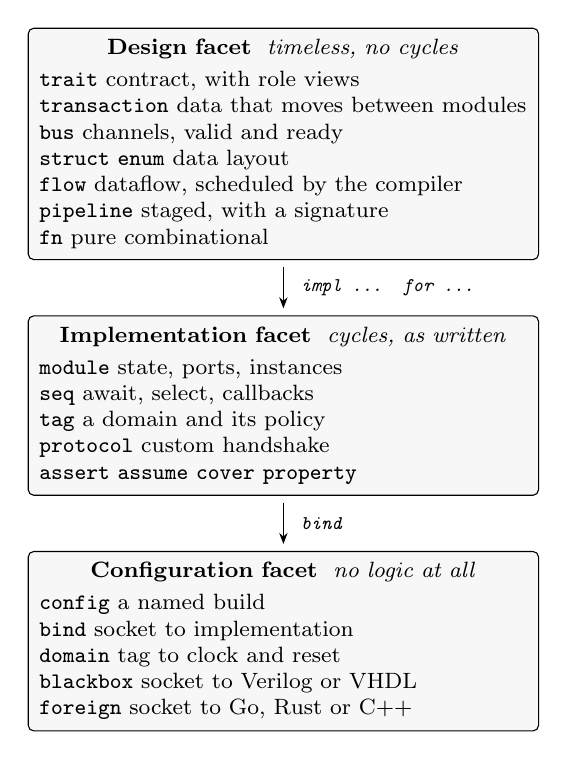
\begin{tikzpicture}[node distance=7mm]

  \node[boxf,text width=62mm,align=left] (design) {%
    \centerline{\textbf{Design facet}\ \ \emph{timeless, no cycles}}\\[2pt]
    \code{trait} contract, with role views \\
    \code{transaction} data that moves between modules \\
    \code{bus} channels, valid and ready \\
    \code{struct} \code{enum} data layout \\
    \code{flow} dataflow, scheduled by the compiler \\
    \code{pipeline} staged, with a signature \\
    \code{fn} pure combinational};

  \node[boxf,text width=62mm,align=left,below=of design] (impl) {%
    \centerline{\textbf{Implementation facet}\ \ \emph{cycles, as written}}\\[2pt]
    \code{module} state, ports, instances \\
    \code{seq} await, select, callbacks \\
    \code{tag} a domain and its policy \\
    \code{protocol} custom handshake \\
    \code{assert} \code{assume} \code{cover} \code{property}};

  \node[boxf,text width=62mm,align=left,below=of impl] (config) {%
    \centerline{\textbf{Configuration facet}\ \ \emph{no logic at all}}\\[2pt]
    \code{config} a named build \\
    \code{bind} socket to implementation \\
    \code{domain} tag to clock and reset \\
    \code{blackbox} socket to Verilog or VHDL \\
    \code{foreign} socket to Go, Rust or C++};

  \draw[fl] (design) -- node[lbl,right=1mm] {\code{impl ... for ...}} (impl);
  \draw[fl] (impl)   -- node[lbl,right=1mm] {\code{bind}} (config);

\end{tikzpicture}
\caption{The three facets and what each one holds. A construct belongs to
exactly one, and the arrows are the only two ways a facet reaches the one
below it.}
\label{fig:facets}
\end{figure}

The rule that makes this work is that a socket in the design facet names a
trait, never an implementation. Both an unbound socket and a directly
instantiated component are legal, and they differ in when the implementation
is chosen. The first defers the choice to a configuration. The second makes
it at the instantiation site.

% SPDX-License-Identifier: Apache-2.0
\section{Surface Syntax, Biased Toward Rust}
\label{sec:syntax}

Where the source languages disagree and Rust provides an established precedent,
the unified specification adopts Rust syntax. Rust syntax provides strong
familiarity, concise expression, and robust scoping rules. Adopting this
convention also yields a decisive structural benefit: it resolves six
grammatical ambiguities present in the source drafts, detailed in
Section~\ref{sec:defects}.

Where Rust has no direct analogue because a construct addresses hardware-specific
concerns, the unified specification adopts the cleaner construct from the source drafts.

Rust naming conventions apply throughout. Types, traits, buses, transactions,
and modules use \code{CamelCase}. Values, functions, ports, and pipeline stages
use \code{snake\_case}. Constants use \code{SCREAMING\_SNAKE\_CASE}.

\subsection{The decision that does the most work}

TxHDL declares sequential state with \code{var} and combinational paths with
\code{wire}. LHDL argues in its eighth thesis that hardware designers should not
draw this distinction manually. Rust resolves this dichotomy through immutability:

\begin{lstlisting}[caption={A binding and a place. \code{mut} encapsulates the distinction previously drawn between \code{wire} and \code{var}.},label={lst:mut}]
let sum = a + b;            // a binding. Always a + b. A wire.
let mut count: u8 = 0;      // a place. Holds its value. A register.
\end{lstlisting}

\code{mut} specifies whether a named value changes over time, expressing an
architectural design invariant. It does not dictate whether synthesis instantiates
a flip-flop, which remains an implementation retiming decision. This reconciles
LHDL's eighth thesis with TxHDL's principle that variables map to registers
automatically based on usage. Both \code{var} and \code{wire} are retired.

\subsection{Conflicts that Rust settles}

Table~\ref{tab:syntax} lists these resolutions. Two specific syntactic entries
warrant detailed discussion.

\emph{Bit slicing.} LHDL writes a Rust range and TxHDL writes a Verilog
descending pair. The range wins, which is the one place LHDL's spelling is
the more Rust-like of the two.

\emph{Awaiting.} Rust settled on postfix, and postfix chains where prefix
does not. Three of TxHDL's four await forms take it without argument. The
fourth, awaiting a condition, has no Rust ancestor, because Rust has no
cycle to wait for. The proposal is that a boolean is itself awaitable and
completes on the first cycle where it holds, which keeps one rule instead of
two. It reads oddly the first time, which is the argument against it.

\begin{table*}[t]
\caption{Conflicts Rust settles, with the precedent for each.}
\label{tab:syntax}
\centering
\footnotesize
\begin{tabular}{@{}llll@{}}
\toprule
Concern & LHDL & TxHDL & Merged \\
\midrule
Assignment          & \code{x := e}          & \code{x = e}             & \code{x = e} \\
Declaration         & \code{var x: T;}       & \code{var} / \code{wire} & \code{let} / \code{let mut} \\
Match arm           & \code{case P: \{..\}}  & \code{P => \{..\}}       & \code{P => \{..\}} \\
Match default       & \code{default:}        & \code{\_ =>}             & \code{\_ =>} \\
Enum variant        & \code{case Data(u32);} & \code{Add = 0x00,}       & both, comma separated \\
Struct fields       & \code{,} and \code{;}  & \code{;}                 & \code{,} \\
Struct literal      & none                   & \code{\{ .addr = 1 \}}   & \code{Req \{ addr: 1 \}} \\
Function            & \code{func f() -> T}   & \code{func f() -> T}     & \code{fn f() -> T} \\
Multi-cycle call    & none                   & \code{proc}              & \code{async fn} \\
Ternary             & none                   & \code{c ? a : b}         & \code{if c \{a\} else \{b\}} \\
Cast                & \code{u16(x)}          & \code{zext(x)}           & \code{x as u16} \\
Visibility          & \code{pub}             & none                     & \code{pub} \\
Packages            & \code{package a.b;}    & none                     & \code{mod}, \code{use a::b} \\
Generics            & \code{<type T>}        & \code{<T, const N: u32>} & \code{<T, const N: u32>} \\
Bit slice           & \code{w[0..8]}         & \code{w[7:0]}            & \code{w[0..8]}, \code{w[12..=14]} \\
Array type          & \code{u32[16]}         & \code{u32[16]}           & \code{[u32; 16]} \\
Loop                & \code{for (i in 0..n)} & \code{for (i in 0..n)}   & \code{for i in 0..n} \\
Loop step           & none                   & \code{step 4}            & \code{(0..n).step\_by(4)} \\
Labels              & none                   & \code{outer:}            & \code{'outer:} \\
Contract            & \code{implements}      & structural               & \code{trait}, \code{impl T for M} \\
Role                & \code{modport Master}  & \code{.master}           & \code{Bus::Master} \\
Assertion           & none                   & \code{assert c : "m"}    & \code{assert!(c, "m")} \\
Parallel branches   & \code{fork}/\code{join}& none                     & \code{join!(f(), g())} \\
Await               & none                   & \code{await port.req}    & \code{port.req.await} \\
Send                & none                   & \code{port.req <- \{..\}}& \code{port.req.send(..).await} \\
Callback            & none                   & \code{then (r) \{..\}}   & \code{.then(|r| \{..\})} \\
Timeout             & none                   & \code{timeout N else}    & \code{.timeout(N).await} \\
Tag application     & \code{@Sync expr}       & none                     & \code{\#[tag(Sync)]} \\
\bottomrule
\end{tabular}
\end{table*}

\subsection{Where Rust has no answer}

These constructs describe hardware, so the better source wins.

\begin{itemize}
  \item \term{Contract for wires}: \code{bus} with \code{channel}, from
        TxHDL. LHDL's \code{interface} does two jobs at once, a wire bundle
        and an implementation socket, which is why its grammar and its
        examples disagree. Splitting the jobs fixes both.
  \item \term{Contract for behaviour}: \code{trait}, replacing LHDL's
        interface in socket position. Late binding needs a name for a role
        an implementation fills, and that is what a trait is.
  \item \term{Timeless behaviour}: \code{flow}, from LHDL's dataflow model.
  \item \term{Sequenced behaviour}: \code{seq}, from TxHDL's sequence.
  \item \term{Synchronisation}: \code{tag}, from LHDL, spelled as an
        attribute, which states in one place what LHDL's grammar and
        examples spell three different ways.
  \item \term{Clock and reset}: \code{domain} in the configuration facet. A
        clock is a physical fact, and the design facet should not name one.
  \item \term{Late binding and foreign code}: \code{config}, \code{bind},
        \code{blackbox} and \code{foreign}, from LHDL. TxHDL has no
        mechanism at all.
  \item \term{Contiguous memory}: a named type, replacing LHDL's comma
        index. A comma inside brackets is too quiet for a decision that
        changes which primitive the synthesiser infers.
\end{itemize}

% SPDX-License-Identifier: Apache-2.0
\section{The Same Design, Three Ways}
\label{sec:worked-example}

A multiply accumulate unit reads pairs of words from memory, accumulates
their products, and answers over a bus. It is small enough to print and
large enough to need a contract, a protocol body, a tag and a binding.

\subsection{As TxHDL states it today}

TxHDL writes the protocol well and cannot state the tag, the contract or the
binding.

\begin{lstlisting}[caption={The multiply accumulate unit as TxHDL states it today. The protocol reads well; the tag, the contract and the binding cannot be written at all.},label={lst:mac-txhdl}]
module MacUnit {
    port host: MacBus.slave;
    port mem:  MemBus.master;

    var acc: u64 = 0;

    pipeline mac(a: u32, b: u32, prev: u64) -> u64 {
        stage mul { var p = zext<u64>(a) * zext<u64>(b); }
        stage add { return prev + p; }
    }

    sequence main {
        loop {
            var req = await host.request;
            acc = 0;
            for (i in 0..req.count) {
                mem.request <- { .addr = req.addr + i*8,
                                 .write = false };
                var lo = await mem.response;
                mem.request <- { .addr = req.addr + i*8 + 4,
                                 .write = false };
                var hi = await mem.response;
                acc = mac(lo.data[31:0], hi.data[31:0], acc);
            }
            host.response <- { .acc = acc };
        }
    }
}
\end{lstlisting}

\subsection{As LHDL states it today}

LHDL states the contract, the tag and the binding, and has no way to write
the loop. The listing below is where an LHDL author stops.

\begin{lstlisting}[caption={The same unit as LHDL states it today. This is where an LHDL author stops: nothing here reads \code{count} words one after another.},label={lst:mac-lhdl}]
interface MacOp {
    addr  : uint<32>;
    count : uint<8>;
    acc   : uint<64>;

    modport Server { in addr; in count; out acc; }
}

tag @MemFetch with handshake, capacity=8;

pipeline Mac implements MacOp.Server {
    pipe p: u64;
    stage Mul { p := a * b; }
    stage Add { acc := p + acc; }
}

config Build {
    bind Top.mac_unit => Mac;
}
\end{lstlisting}

No LHDL construct reads \code{count} words one after another and waits for
each response. A state machine would state it as hand written states, which
is the form \code{await} exists to replace.

\subsection{Merged}

\begin{lstlisting}[caption={The same unit, merged. Nine differences from the first listing, one per decision in Table~\ref{tab:syntax}.},label={lst:mac-merged}]
transaction MacRequest { addr: u32, count: u8 }
transaction MacResponse { acc: u64 }

bus MacBus {
    channel request:  MacRequest,
    channel response: MacResponse,
}

pub trait MacOp {
    async fn run(&mut self, req: MacRequest) -> MacResponse;
}

// Two stages, so the multiplier does not sit in the adder's
// path. The compiler places the register between them.
pipeline mac(a: u32, b: u32, prev: u64) -> u64 {
    stage mul { let p = (a as u64) * (b as u64); }
    stage add { prev + p }
}

#[tag(MemFetch, handshake, capacity = 8)]
pub module MacUnit {
    port host: MacBus::Slave,
    port mem:  MemBus::Master,

    let mut acc: u64 = 0;

    seq main {
        loop {
            let req = host.request.await;
            acc = 0;

            for i in 0..req.count {
                let lo = mem.read(req.addr + i*8).await;
                let hi = mem.read(req.addr + i*8 + 4).await;
                acc = mac(lo.data[0..32], hi.data[0..32], acc);
            }

            assert!(req.count > 0, "empty accumulate");
            host.response.send(MacResponse { acc }).await;
        }
    }
}

impl MacOp for MacUnit {}

config Build {
    bind top.mac_unit => MacUnit;

    domain MemFetch {
        clock: sys_clk_100mhz,
        reset: sys_rst_n,
    }
}
\end{lstlisting}

Nine specific structural differences distinguish this example from the
original TxHDL implementation, directly reflecting the decisions established
in Table~\ref{tab:syntax}:

\begin{enumerate}
  \item \code{var acc} becomes \code{let mut acc}, so the text says the
        value changes and not that a register exists.
  \item The zero-extension call becomes an \code{as} cast.
  \item The descending bit slice becomes a range.
  \item The prefix await becomes postfix.
  \item The send becomes a call that returns a value, so a request and its
        response are one line instead of two.
  \item The designated initialiser becomes a struct literal, with the type
        named and field shorthand doing the rest.
  \item \code{sequence} becomes \code{seq}, and its cycle counts stay
        exactly as written.
  \item The tag, the trait and the configuration come from LHDL, and TxHDL
        had no way to write any of them.
  \item The assertion comes from TxHDL, and LHDL had no way to write it.
\end{enumerate}

% SPDX-License-Identifier: Apache-2.0
\section{Defects in the Sources}
\label{sec:defects}

These were found by reading, because no parser exists for either language.
Each has to be settled while merging, since a merged specification cannot
state two things at once.

\subsection{TxHDL}

Eleven, in \code{spec/language.md}. The line numbers are from the file as
committed.

\begin{itemize}
  \item Line 1: the file begins with the literal text \code{:qODq} before
        its title. A stray editor keystroke was committed, and it rendered
        into the title of the first PDF built from the file.
  \item Line 660 states that a module holds only one sequence.
        \code{module Counter} at line 416 declares two, and
        \code{module DualPortMemory} at line 2012 declares two.
  \item Lines 133 and 141: inside one enumeration, two variants share the
        encoding \code{0x02}. Lines 135 and 140 share \code{0x04}.
  \item Line 1112: an array declared with 256 elements is initialised with
        four and a comment.
  \item Line 740: a timeout requires its else block to end in a value, and
        blocks as expressions are never defined.
  \item Line 2043: a port uses an anonymous bus type inline, and the bus
        section never defines that form.
  \item Line 1196: a clock domain is given a frequency literal, and the
        literal section defines no unit suffix.
  \item There is no grammar. A quick reference lists keywords and
        operators, and never their syntax.
  \item Transactions and structs are both product types, with no stated
        rule for choosing one.
  \item Subtype compatibility says a receiver ignores extra fields, and the
        width of the physical channel for that case is not stated.
\end{itemize}

\subsection{LHDL}

The grammar and the examples disagree in sixteen places. Three are enough on
their own: no interface, no modport and no generic parameter list written in
any of the four LHDL files parses against the grammar in the condensed
specification.

\begin{itemize}
  \item An interface item must be a directed port declaration, and every
        interface in every file writes undirected fields.
  \item A modport takes port declarations, which require a type, and every
        modport writes a direction and a name with no type.
  \item A generic declaration puts the name first, and the examples write
        the keyword first.
  \item A tag definition requires a type, and five examples omit it. One
        writes the tag name with a leading marker the grammar does not
        allow. Another writes a comma the grammar does not allow.
  \item A variable declaration has no initialiser, and the examples give
        one.
  \item The parallel-composition statement has two incompatible
        productions, one per file. Every example uses the first.
  \item The operator table offers two assignment operators, and the grammar
        offers one.
  \item A state transition takes a keyword in the grammar, and one example
        omits it.
  \item The prose names functions one way and the grammar another.
  \item Struct fields are comma separated in the grammar and semicolon
        separated in one example.
  \item A module has no port list and no tag in the grammar, and one
        example gives it both.
  \item Neither the domain block nor a bare binding appears among the
        top-level definitions, and both appear at top level in an example.
  \item An instance declaration requires a parenthesised binding list, and
        an example has none.
  \item One example calls an interface instance as a function, and no rule
        covers that.
\end{itemize}

The LL(1) claim is asserted and never checked. One conflict is visible
without tooling: two top-level productions both begin with an optional
\code{pub}, so a predictive parser cannot choose between them on that token
until the prefix is factored out.

\subsection{Lessons for the unified specification}

Both original source drafts include grammars or syntactic claims that diverge
from their own code listings. This divergence persisted because neither draft
was verified by automated tooling. In the unified specification, every
syntactic construct possesses a corresponding reference example in a standalone
file verified by automated test harnesses. This practice enforces the project
requirement that every specification construct must be accompanied by a
passing automated test.

% SPDX-License-Identifier: Apache-2.0
\section{Decisions and Remaining Work}
\label{sec:decisions}

\subsection{Settled}

\emph{The name is TxHDL.} The repository, the build module and the published
path are all named \code{txhdl}, and transactions are the distinguishing
idea. FLHDL, LHdl and LHDL are retired, and appear from here on only in the
project's analysis documents.

\emph{The behavioural keywords are \code{flow} and \code{seq}.} Selecting
neutral terminology establishes clear semantic separation from legacy
constructs in both progenitor drafts.

\emph{The disposition of legacy LHDL source files is deferred.} These
documents remain in the repository as historical reference material.
The twelve foundational design theses are incorporated into the unified
document within a dedicated architectural rationale section.

\subsection{Still open}

\begin{itemize}
  \item \emph{Awaiting conditions.} Permitting boolean expressions to implement
        the awaitable interface preserves a single syntax rule, whereas
        introducing a dedicated statement adds specialized syntax for a single
        use case.
  \item \emph{Chaining.} Replacing LHDL's pipe operator with a method chain
        costs one non-Rust operator and reads well for long chains either
        way.
  \item \emph{Whether a transaction is its own item} or an attribute on a
        struct. The attribute is one fewer keyword at the cost of a longer
        declaration.
\end{itemize}

\subsection{Order of work}

\begin{enumerate}
  \item Write the merged specification section by section, in facet order,
        taking the type system and the bit manipulation set first, because
        nothing else can be written without them.
  \item Write the grammar as each section lands, rather than at the end, and
        check the LL(1) property with a generator instead of asserting it.
  \item Fold the facets, tags and configuration in from LHDL.
  \item Fold the twelve theses in as a rationale section.
  \item Move every code example out of the prose and into its own file, so
        the examples become a test corpus.
\end{enumerate}

The second step matters most, for the reason
Section~\ref{sec:defects} gives.

% SPDX-License-Identifier: Apache-2.0
\section{Conclusion}
\label{sec:conclusion}

Two hardware description languages developed independently for the same
project proved to represent complementary facets of a unified architecture.
LHDL specifies system assembly, static configuration, and dataflow scheduling,
yet provides no primitives for multi-cycle protocol sequencing. TxHDL specifies
cycle-accurate transaction handling within modules, yet provides no mechanisms
for system-level interconnect composition. The unified specification retains
both domains.

Only four issues required semantic decisions rather than syntactic reconciliation.
Among these, reconciling the model of time is foundational: both models are
correct within their respective operating boundaries. Cycle counts mandated by
external bus protocols represent architectural specifications, whereas latency
arising from target fabric timing represents an implementation parameter.

Surface syntax aligns with Rust, establishing consistent conventions while
eliminating six grammatical defects present in the source drafts. The remaining
grammatical ambiguities are resolved through automated verification, ensuring
that every construct in the unified TxHDL specification is backed by passing
test suites.


\begin{thebibliography}{10}

\bibitem{ieee1076}
IEEE, \emph{IEEE Standard VHDL Language Reference Manual}, IEEE Std
1076-2019, 2019.

\bibitem{ieee1800}
IEEE, \emph{IEEE Standard for SystemVerilog}, IEEE Std 1800-2023, 2023.

\bibitem{carloni2001}
L.~P. Carloni, K.~L. McMillan, and A.~L. Sangiovanni-Vincentelli, ``Theory of
latency-insensitive design,'' \emph{IEEE Trans. Computer-Aided Design},
vol.~20, no.~9, pp. 1059--1076, 2001.

\bibitem{cortadella2006}
J.~Cortadella, M.~Kishinevsky, and B.~Grundmann, ``Synthesis of synchronous
elastic architectures,'' in \emph{Proc. Design Automation Conf.}, 2006, pp.
657--662.

\bibitem{bachrach2012}
J.~Bachrach \emph{et al.}, ``Chisel: Constructing hardware in a Scala embedded
language,'' in \emph{Proc. Design Automation Conf.}, 2012, pp. 1216--1225.

\bibitem{nikhil2004}
R.~Nikhil, ``Bluespec System Verilog: efficient, correct RTL from high level
specifications,'' in \emph{Proc. MEMOCODE}, 2004, pp. 69--70.

\bibitem{rust}
N.~D. Matsakis and F.~S. Klock, ``The Rust language,'' \emph{Ada Letters},
vol.~34, no.~3, pp. 103--104, 2014.

\end{thebibliography}

\end{document}
